\chapter{Requisiti Funzionali}
\label{ch:requisitiFunzionali}

Di seguito vengono riportati i requisiti funzionali (\texttt{RF}) del programma "SatisTrento" tramite \textit{Use Case Diagram} (\texttt{UCD}) progettati usando il linguaggio \texttt{UML}.

% Esempio di markup
\section{\underline{Utente Anonimo}}
    Di seguito i requisiti associati all'Utente Anonimo:
    \begin{itemize}
        \item \textbf{RF1}: Mappa
        \item \textbf{RF2}: Multi lingua
        \item \textbf{RF3}: Accesso dati zona selezionata
        \item \textbf{RF4}: Accesso dati specifici zona selezionata
    \end{itemize}
    \begin{figure}[H]
        \centering
        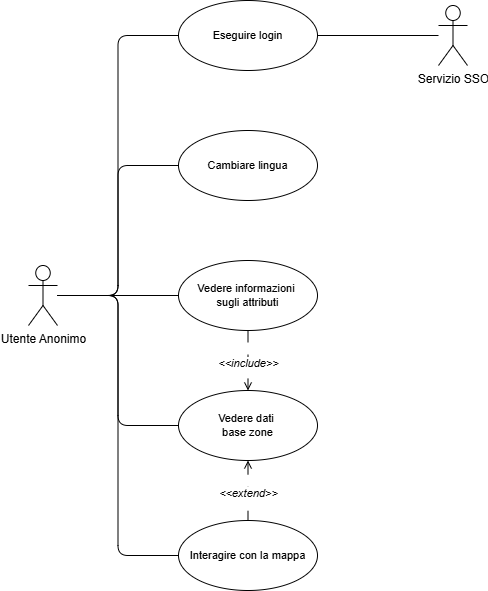
\includegraphics[width=0.8\textwidth]{UseCase_diagrams/Utente_Anonimo.drawio.png}
        \caption{Use Case Diagram dell'Utente anonimo}
    \end{figure}
    \subsection{Use Case {RF1}: Mappa}
        \subsubsection{Riassunto}
            Questo Use Case descrive come l'utente potrà interagire con la mappa
        \subsubsection{Descrizione}
            \begin{itemize}
            \item L'utente anonimo posiziona il cursone all'interno dello spazio dedicato alla mappa
            \item Attraverso l'utilizzo della rotella del mouse o dei pulsanti prensenti in uno degli angoli della mappa l'utente potrà rimpicciolire o ingrandire la dimensione dello zoom sulla mappa
            \item L'utente premendo e trascinando il cursore si sposta all'interno della mappa
            \item L'utente premendo su di una zona selezionerà la stessa portando alla visualizzazione della zona delezionata (RF3)
            \end{itemize}
        \subsubsection{Eccezioni}
            1. Se l'utente clicca su di un quartiere già selezionato questo riporterà alla visualizzazione della Homepage (RF1)
        \subsubsection{Estensioni}
            Estensioni del requisito uno    % Da discutere il concetto dell'estensione per quanto riguarda l'RF2
    \subsection{Use Case {RF2}: Multi lingua}
        \subsubsection{Riassunto}
            Questo Use Case descrive come l'utente potrà cambiare la lingua dei vari testi presenti nel programma
        \subsubsection{Descrizione}
            \begin{enumerate}
            \item L'utente premendo su di una delle bandiere presenti nella header cambierà la selezione della lingua
            %da finire
            \end{enumerate}
        \subsubsection{Eccezioni}
            %to-do
        \subsubsection{Estensioni}
            %non penso ci siano ma to-do